\documentclass[11pt,a4paper]{article}
\usepackage[utf8]{inputenc}
\usepackage[T1]{fontenc}
\usepackage{lmodern}
\usepackage[english]{babel}
\usepackage{amsmath,amssymb}
\usepackage{booktabs}
\usepackage{graphicx}
\usepackage{adjustbox}
\usepackage{xcolor}
\usepackage{url}
\usepackage[margin=2.4cm,headheight=14pt]{geometry}
\usepackage[numbers,sort&compress]{natbib}
\usepackage{microtype}
\usepackage{enumitem}
\usepackage{tikz}
\usetikzlibrary{positioning,arrows.meta,calc,fit,backgrounds}
\usepackage[most]{tcolorbox}
\usepackage{titlesec}
\usepackage{fancyhdr}
\usepackage{caption}
\usepackage[hidelinks]{hyperref}

% house style (AIgen Solutions working papers)
\definecolor{aigen}{HTML}{1F4E8C}
\definecolor{accent}{HTML}{D9742B}
\definecolor{abstractbg}{HTML}{F3F6FB}
\definecolor{muted}{HTML}{6B6B6B}
\titleformat{\section}{\sffamily\bfseries\Large\color{aigen}}{\thesection}{0.8em}{}
\titleformat{\subsection}{\sffamily\bfseries\large\color{aigen}}{\thesubsection}{0.8em}{}
\titleformat{\paragraph}[runin]{\bfseries}{}{0em}{}
\titlespacing*{\section}{0pt}{1.6ex plus .6ex minus .2ex}{0.9ex}
\titlespacing*{\subsection}{0pt}{1.2ex plus .4ex}{0.6ex}
\captionsetup{labelfont={bf,color=aigen},font=small,labelsep=period}
\pagestyle{fancy}\fancyhf{}
\lhead{\small\sffamily\color{muted}Leak Rate, Not Loss}
\rhead{\small\sffamily\bfseries\color{aigen}LeakIT}
\lfoot{\small\sffamily\color{muted}Working paper \textperiodcentered\ November 2026 \textperiodcentered\ AIgen Solutions}
\rfoot{\small\sffamily\thepage}
\renewcommand{\headrulewidth}{0.3pt}
\setlength{\parskip}{0.35em}
\newtcolorbox{abstractbox}{enhanced,breakable,colback=abstractbg,colframe=aigen,boxrule=0pt,leftrule=2.5pt,arc=0pt,left=9pt,right=9pt,top=7pt,bottom=7pt,fontupper=\small}
\newtcolorbox{numbersbox}{enhanced,colback=white,colframe=aigen,boxrule=0.5pt,arc=0pt,left=6pt,right=6pt,top=8pt,bottom=8pt}
\newcommand{\keynumber}[3]{\begin{minipage}[t]{0.31\textwidth}\centering{\sffamily\bfseries\huge\color{#1}#2}\\[2pt]{\small #3}\end{minipage}}

\newcommand{\TBD}[1]{\textcolor{red!70!black}{[#1]}}
\newcommand{\pseud}[1]{\texttt{#1}}
\newcommand{\dprime}{d'}

\begin{document}
\thispagestyle{empty}
\noindent{\sffamily\bfseries\small\color{aigen}WORKING PAPER \textperiodcentered\ PREPRINT EDITION}\hfill{\sffamily\small\color{muted}5 NOVEMBER 2026 \textperiodcentered\ VERSION 1.0}

\vspace{1.4em}
{\noindent\sffamily\bfseries\fontsize{22}{27}\selectfont\color{aigen}Leak Rate, Not Loss:\\ Measuring What Actually Escapes\\ When a Local Model Pseudonymizes\\ Text for Frontier LLMs\par}

\vspace{0.9em}\noindent{\color{aigen}\rule{\textwidth}{0.5pt}}

\vspace{0.7em}
{\noindent\sffamily\large Alessio Rocchi\par}
{\noindent\sffamily\small\color{muted}AIgen Solutions\par}
{\noindent\sffamily\small\color{aigen}PII leak rate \textperiodcentered\ pseudonymization \textperiodcentered\ LLM re-identification \textperiodcentered\ Italian benchmark\par}

\vspace{1.1em}
\begin{abstractbox}
{\sffamily\bfseries\color{aigen}Abstract}\par\vspace{0.35em}
Enterprises routinely reject frontier LLM APIs on data-protection grounds, yet the alternative, small on-premise models, underperforms on non-trivial tasks at comparable cost. A common compromise places a local model in front of the API to replace personal identifiers with typed pseudonyms (e.g.\ \pseud{PER\_f\_0012}) and reverses the mapping on output. Prior work evaluates such pipelines by downstream task quality; we argue this is the wrong metric, since quality loss is negligible by construction while the actual risk, identifiers that survive pseudonymization, is never measured. We define \emph{leak rate} per identifier category with cluster-bootstrap confidence intervals, release \textsc{LeakIT}, an Italian benchmark of 2\,000 synthetic free-text documents (legal, financial, HR, clinical; 400 held-out test documents) with character-level ground truth for direct and quasi-identifiers, and evaluate five local pseudonymizers (a regex baseline, Microsoft Presidio with the Italian spaCy pipeline, their hybrid, GLiNER, and a fine-tuned Italian encoder) against three frontier models (Claude Opus, Sonnet and Haiku~5.5) used as their own anonymizers. We further measure re-identification risk from surviving quasi-identifiers both as $k$-anonymity on what is still readable and as what an LLM attacker actually infers, and downstream quality on four tasks for three consumer models and three replacement policies. Results on the test split: the standard off-the-shelf configuration (Presidio + regex, typed pseudonyms) lets at least one direct identifier through in 41.2\,\% of documents (95\,\% CI 36.5--46.2) and zero-shot GLiNER in 93.8\,\%; normalizing the case of the detector's input, a preprocessing step with no training, halves Presidio's rate to 19.5\,\% and brings a supervised multilingual NER model (WikiNEuRal) to 11.0\,\% [8.2, 14.2]. The frontier models asked to anonymize their own input leak 0.0--0.2\,\%; an encoder fine-tuned on the benchmark leaks 0.0\,\% in and across domains but at twenty times the over-redaction, a number we report as a property of the synthetic data rather than as a result. The leak is almost entirely person names (18.2\,\% of mentions), concentrated in surname-only (38.6\,\%), all-caps (32.8\,\%) and \emph{SURNAME Name} (20.9\,\%) forms that Italian legal and HR documents use constantly; structured identifiers (codice fiscale, IBAN, partita IVA, e-mail, phone) leak at 0\,\% once validated patterns are added. An LLM attacker recovers the subject's surname from 35\,\% of the pseudonymized documents and places 14\,\% of subjects in an estimated population class of fewer than 11 under ISTAT marginals (64\,\% on raw text, 2\,\% after perfect pseudonymization). Downstream, typed pseudonyms cost the consumer 0.4 points on QA, 2.5 on extraction and 3.8 on classification; with gold-span pseudonymization the cost is zero, so the loss is the detector's, not the pseudonym's. Typed pseudonyms do not reduce grammatical-agreement errors (below 2\,\% either way) but double the share of pseudonyms the model dares to gender. We discuss the GDPR status of the pipeline (pseudonymization under Art.~4(5), the relative reading of identifiability after \emph{EDPS v SRB}, C-413/23~P) and what a DPIA must document. Code, data and mapping schema are public.
\end{abstractbox}

\vspace{0.6em}
\begin{numbersbox}
\keynumber{aigen}{41.2\,\%}{of test documents still carry a direct identifier after the standard local stack (Presidio + regex); 11.0\,\% with case normalization and a supervised multilingual NER, no training}\hfill
\keynumber{aigen}{35\,\%}{of pseudonymized documents from which an LLM attacker recovers the subject's surname}\hfill
\keynumber{accent}{0 / 1\,717}{structured identifiers (fiscal codes, IBANs, VAT numbers, e-mails, phones, document numbers, plates) that leak once validated patterns are added}
\end{numbersbox}

\vspace{0.5em}
\noindent{\sffamily\bfseries\small Keywords:} {\small pseudonymization; PII detection; leak rate; $k$-anonymity; LLM re-identification; GDPR; Italian; benchmark.}

\vspace{0.4em}
\noindent{\sffamily\bfseries\scriptsize AI use disclosure.} {\scriptsize AI systems supported the literature search, code drafting, experiment orchestration, analysis validation and language and visual editing under human supervision. The author verified the sources, methods, results and final manuscript and retains responsibility for the work. Code, data, prompts and the call cache are released with the paper.}

\vspace{0.8em}
\begin{figure}[h]
\centering
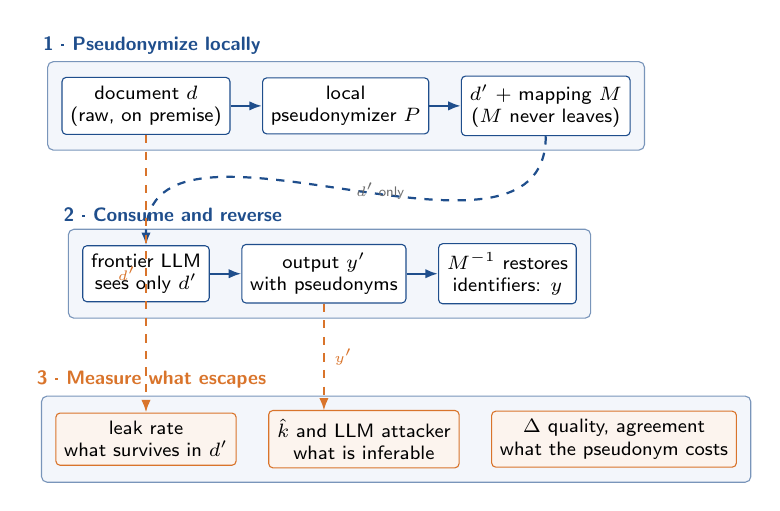
\begin{tikzpicture}[font=\sffamily\scriptsize, node distance=4mm,
  box/.style={draw=aigen, fill=white, rounded corners=1.5pt, inner sep=3pt, minimum height=5.5mm, align=center},
  warn/.style={draw=accent, fill=accent!8, rounded corners=1.5pt, inner sep=3pt, minimum height=5.5mm, align=center},
  panel/.style={draw=aigen!60, fill=abstractbg, rounded corners=2pt, inner sep=5pt},
  arr/.style={-{Latex[length=1.6mm]}, aigen, thick}]
  % panel 1
  \node[box] (d) {document $d$\\(raw, on premise)};
  \node[box, right=of d] (P) {local\\pseudonymizer $P$};
  \node[box, right=of P] (dp) {$\dprime$ + mapping $M$\\($M$ never leaves)};
  \draw[arr] (d) -- (P); \draw[arr] (P) -- (dp);
  % panel 2
  \node[box, below=14mm of d] (llm) {frontier LLM\\sees only $\dprime$};
  \node[box, right=of llm] (yp) {output $y'$\\with pseudonyms};
  \node[box, right=of yp] (y) {$M^{-1}$ restores\\identifiers: $y$};
  \draw[arr] (llm) -- (yp); \draw[arr] (yp) -- (y);
  % panel 3
  \node[warn, below=14mm of llm] (leak) {leak rate\\what survives in $\dprime$};
  \node[warn, right=of leak] (k) {$\hat k$ and LLM attacker\\what is inferable};
  \node[warn, right=of k] (q) {$\Delta$ quality, agreement\\what the pseudonym costs};
  \begin{scope}[on background layer]
    \node[panel, fit=(d)(P)(dp), label={[font=\sffamily\bfseries\scriptsize, aigen, anchor=south west, xshift=-5pt, yshift=-1pt]north west:1 \textperiodcentered\ Pseudonymize locally}] (p1) {};
    \node[panel, fit=(llm)(yp)(y), label={[font=\sffamily\bfseries\scriptsize, aigen, anchor=south west, xshift=-5pt, yshift=-1pt]north west:2 \textperiodcentered\ Consume and reverse}] (p2) {};
    \node[panel, fit=(leak)(k)(q), label={[font=\sffamily\bfseries\scriptsize, accent, anchor=south west, xshift=-5pt, yshift=-1pt]north west:3 \textperiodcentered\ Measure what escapes}] (p3) {};
  \end{scope}
  \draw[arr, dashed] (dp.south) to[out=-90, in=90] node[midway, right, muted, font=\sffamily\tiny] {$\dprime$ only} (llm.north);
  \draw[arr, dashed, accent] (d.south) -- node[midway, left, accent, font=\sffamily\tiny] {$\dprime$} (leak.north -| d.south);
  \draw[arr, dashed, accent] (yp.south) -- node[midway, right, accent, font=\sffamily\tiny] {$y'$} (q.north -| yp.south);
\end{tikzpicture}
\caption{The pipeline and what this paper measures. The mapping $M$ stays on premise; the provider receives only $\dprime$. Prior work evaluates the pipeline by panel 2 alone. The three quantities of panel 3 are computed on $\dprime$ and on $y'$, with confidence intervals over documents.}
\label{fig:pipeline}
\end{figure}

\section{Introduction}
\label{sec:intro}

The deployment pattern this paper studies is simple. A document $d$ containing personal data is handed to a small model running on the organisation's own hardware; that model replaces every personal identifier it finds with a pseudonym, producing $\dprime$ and a mapping $M$ that never leaves the premises; $\dprime$ is sent to a frontier LLM together with a task; the LLM's output $y'$ is passed through $M^{-1}$ to restore the identifiers. The provider sees only $\dprime$ and $y'$. The pattern is attractive because it lets regulated organisations buy frontier-model quality while telling their data-protection officer that no personal data leaves the building.

That sentence is true exactly to the extent that the local model finds every identifier. The literature on this pattern has largely measured something else. Work on pseudonymization for NLP pipelines \citep{yermilov2023pseudonymization,chen2023has} and on LLM-based anonymizers \citep{staab2024anonymizers} reports downstream task quality (summarization ROUGE, extraction F1, classification accuracy) under pseudonymization, and finds, unsurprisingly, that it barely changes. Quality is preserved \emph{by construction}: a typed pseudonym carries the information the downstream task needs (that this token is a person, a company, a city) and removes only the information it does not. The quantity that decides whether the deployment is lawful and safe is the complement: how much of what should have been removed is still in $\dprime$.

We call that quantity the \emph{leak rate} and make five claims.

\begin{enumerate}[nosep]
\item \textbf{Leak rate is the primary metric}, downstream quality a sanity check. We define leak rate per identifier category at mention, entity and document level (\S\ref{sec:leak}), with confidence intervals that respect the clustering of mentions inside documents (\S\ref{sec:ci}); the mention-level Wilson interval that would normally be reported understates uncertainty.
\item \textbf{Off-the-shelf local pseudonymization leaks a lot, and it leaks names.} On a 400-document Italian test set spanning legal, financial, HR and clinical text, Presidio with the Italian spaCy pipeline plus validated regular expressions leaves at least one direct identifier in 41\,\% of documents. Structured identifiers are essentially solved; person names in the forms that Italian institutional prose actually uses (\emph{ROSSI Mario}, \emph{il sig.\ Rossi}, \emph{MARIO ROSSI}) are not (\S\ref{sec:results}). Normalizing the case of the detector's input, a preprocessing step that costs nothing, halves the document leak rate to 19.5\,\%; the same step in front of a supervised multilingual NER model brings it to 11.0\,\%.
\item \textbf{What survives is enough to single people out.} Even when direct identifiers are removed, the quasi-identifiers a task needs (age, profession, diagnosis) combined with those the pseudonymizer missed (employer, city) leave 12.5\,\% of data subjects in an estimated population equivalence class of fewer than 11 (\S\ref{sec:kanon}). This is the quantity a GDPR Art.~35 impact assessment must document, and it is not derivable from an F1 score. An LLM attacker given the pseudonymized text recovers the surname in 35\,\% of documents and reaches the same $\hat k$ distribution as the surface count (\S\ref{sec:attacker}): what is readable is what is inferable.
\item \textbf{Most of the gap closes with preprocessing, not training.} Case-normalizing the detector's input halves Presidio's leak and takes a supervised multilingual NER model to 11\,\%; zero-shot GLiNER leaks in 94\,\% of documents whatever the preprocessing. A BERT encoder fine-tuned on the benchmark leaks 0\,\% in and across domains, but we report that as a property of the synthetic data (closed vocabulary, shared template families, a twenty-fold rise in over-redaction across domains), not as a result; the three frontier models asked to anonymize their own input also leak 0.0--0.2\,\%.
\item \textbf{Downstream loss is the detector's, not the pseudonym's.} Typed pseudonyms cost Opus~5.5 $0.4$ points on QA, $2.5$ on extraction and $3.8$ on classification; with gold-span replacement the cost is $0.0$ and $+1.8$. Typed and opaque pseudonyms are indistinguishable on quality; what typed pseudonyms change is that the model writes gendered Italian at all (41--43\,\% of pseudonyms against 22--24\,\%), not how often it gets the gender wrong ($<2$\,\% either way).
\end{enumerate}

Because real Italian legal, HR and clinical documents cannot be released, we built a seeded generator that produces realistic documents with character-level ground truth and valid checksums for every Italian structured identifier (\S\ref{sec:data}). The generator, benchmark, pseudonymizer adapters, metrics and the mapping schema are released so that the same measurements can be made on a private corpus without changing a line of the evaluation code.

\section{Related work}
\label{sec:related}

\paragraph{Text anonymization and its evaluation.} \citet{lison2021anonymisation} survey anonymization models for text and argue that NER-style evaluation (precision/recall on spans) does not measure privacy. The Text Anonymization Benchmark \citep{pilan2022tab} introduces entity-level recall on direct and quasi-identifiers with human annotations of what \emph{needs} masking, and \citet{mozes2021nointruder} propose evaluating against an intruder. Our leak rate is in this family: it is one minus recall, measured on the output text rather than on predicted spans, but with three differences relevant to the deployment: it is computed on the \emph{text the provider receives}, so a span that is mis-typed but still replaced counts as protected; it has a partial-leak variant for discriminating fragments; and its uncertainty is estimated by resampling documents.

\paragraph{De-identification of clinical text.} The i2b2/UTHealth shared tasks \citep{stubbs2015i2b2} and transformer-based de-identifiers \citep{johnson2020deid} established high recall on English clinical PHI. Italian clinical text has no comparable public resource; our clinical domain is a synthetic stand-in with the identifier categories of those tasks.

\paragraph{PII detectors.} Presidio \citep{presidio} is the de-facto open-source default and ships Italian recognizers for fiscal code, VAT, identity card, passport and driving licence; its NER comes from spaCy \citep{spacy_it}. GLiNER \citep{zaratiana2024gliner} offers zero-shot NER with prompted labels and is increasingly used as a PII detector. \citet{mansfield2022behind} show that name detection for PII masking is demographically biased; our per-form analysis (\S\ref{sec:results}) shows an orthographic analogue: the same name is or is not found depending on casing and order.

\paragraph{Pseudonymization for LLM pipelines.} \citet{yermilov2023pseudonymization} and HaS \citep{chen2023has} study replacing entities before sending text to a model and restoring them after, and evaluate by task quality. \citet{staab2024anonymizers} use an LLM adversary to anonymize against inference attacks, following \citet{staab2024beyond} who show that LLMs infer personal attributes from text at scale; this is the quasi-identifier risk we quantify with $k$-anonymity rather than with an adversarial model. \citet{dou2024selfdisclosure} target self-disclosures in user text. None of these report the share of identifiers that survive in the text sent to the provider as the headline metric.

\paragraph{Re-identification benchmarks with an LLM attacker.} Closest to our setting, RAT-Bench \citep{krco2026ratbench} scores anonymizers (NER-based ones such as Presidio and LLM-based ones) by the re-identification risk an LLM attacker achieves on synthetic texts generated from U.S.\ demographic statistics, and finds LLM-based anonymizers to offer the better privacy--utility trade-off at higher cost. We share the synthetic-from-marginals construction and the LLM attacker (\S\ref{sec:attacker}), and differ in four places: the texts are Italian institutional documents with the full identifier set (fiscal code, IBAN, VAT, plates) and their real orthographic variety; the primary metric is the verbatim leak rate of direct identifiers with a document-level CI, with inference-based risk as the second layer rather than the only one; the anonymizer is a reversible typed pseudonymizer whose mapping stays on-premise, so grammatical agreement and reverse mapping are part of the measurement; and the comparison that matters for the deployment, a local model versus the frontier model as its own anonymizer, is explicit. \citet{lermen2026deanonymization} show that an LLM agent re-identifies pseudonymous users at scale (67\,\% recall at 90\,\% precision on Hacker News against LinkedIn, for a few dollars per target), which is the attacker our $\hat k$ should be read against. \citet{xiao2026saysomething} find that free-text pseudonymization gives the best privacy--utility trade-off among drafting strategies for LLM agents, and that single-message evaluation underestimates leakage.

\paragraph{Re-identification risk.} $k$-anonymity \citep{sweeney2002} and $l$-diversity \citep{machanavajjhala2007} were defined for tabular microdata; we apply them to the quasi-identifier tuple that can be read off a pseudonymized document, following the ``what can the recipient do with it'' framing of the Anonymisation Decision-Making Framework \citep{elliot2016adf}.

\section{Pipeline, threat model and definitions}
\label{sec:defs}

\subsection{Pipeline}
A local pseudonymizer $P$ maps $d \mapsto (\dprime, M)$. $M$ is a list of entries (pseudonym, category, canonical value, surface forms, attributes). Pseudonyms are \emph{typed}: $\pseud{<TYPE>\_<attrs>\_<counter>}$, e.g.\ \pseud{PER\_f\_0012}, \pseud{ORG\_0002}, \pseud{CF\_0001}. The type tells the downstream model what kind of thing the token is; for persons the gender attribute (\pseud{m}/\pseud{f}, \pseud{x} if unknown) lets it produce grammatical Italian (``la dott.ssa \pseud{PER\_f\_0012} è stata convocata''). Counters are per document and per type, assigned in order of first appearance, so a pseudonym is not a cross-document identifier. The control condition uses \emph{opaque} pseudonyms, 8-hex-digit tokens \pseud{[[a3f9c2e1]]} carrying neither type nor gender. All pseudonymizers under test share the post-detection machinery (overlap resolution, coreference linking, pseudonym assignment, rewriting) so that they differ only in what they detect.

\subsection{Threat model}
The adversary is the provider, or anyone with access to its logs. It sees $\dprime$ and $y'$ and does not see $M$. We make no assumption about its background knowledge beyond public reference data (population registers, company registers), which is what the $k$-anonymity estimate uses. A \emph{leak} is any ground-truth identifier mention of $d$ whose surface form, or an informative fragment of it, is still present in $\dprime$.

\subsection{Identifier categories}
Direct identifiers (identify the data subject alone): \pseud{PER} (person name in any surface form), \pseud{CF} (codice fiscale), \pseud{IBAN}, \pseud{PIVA} (partita IVA), \pseud{EMAIL}, \pseud{PHONE}, \pseud{ADDRESS} (street and number), \pseud{DOC\_ID} (identity card, passport, licence number), \pseud{PLATE}, \pseud{DATE\_BIRTH}. Quasi-identifiers (identify in combination): \pseud{ORG} (employer, counterparty), \pseud{LOC} (city, nationality), \pseud{AGE}, \pseud{PROFESSION}, \pseud{HEALTH} (diagnosis, drug; special-category data under Art.~9 GDPR), \pseud{DATE} (other dates).

\subsection{Leak rate}
\label{sec:leak}
Let $G_c$ be the multiset of ground-truth mentions of category $c$ in the corpus and $\dprime_i$ the pseudonymized text of document $i$. A mention $m\in G_c$ with surface $s$ and canonical value $v$ leaks \emph{strictly} if $\mathrm{norm}(s)$ occurs in $\mathrm{norm}(\dprime_i)$ as a token-bounded substring, where $\mathrm{norm}$ lower-cases, strips diacritics and, for numeric identifiers, removes separators (so \pseud{IT60 X054 2811 \ldots} matches \pseud{IT60X0542811\ldots}); dates are matched in every common Italian rendering. It leaks \emph{partially} if a discriminating fragment of $v$ survives: the surname token for \pseud{PER}, the first six or last five characters of a \pseud{CF} (surname/name encoding; birthplace and check), the last twelve digits of an \pseud{IBAN}, the last seven digits of a \pseud{PHONE}, the local part of an \pseud{EMAIL}, street name and number for an \pseud{ADDRESS}, day and month or the year for a \pseud{DATE\_BIRTH}. We report
\begin{align*}
\mathrm{leak}(c) &= \frac{|\{m\in G_c : m \text{ leaks strictly}\}|}{|G_c|}, \qquad
\mathrm{leak}_{\partial}(c) = \frac{|\{m\in G_c : m \text{ leaks strictly or partially}\}|}{|G_c|},\\
\mathrm{docleak} &= \frac{|\{i : \exists\, \text{direct mention in } d_i \text{ that leaks strictly}\}|}{N},
\end{align*}
plus an \emph{entity-level} rate (an entity leaks if any of its mentions does; the right unit for re-identification) and an \emph{over-redaction} rate (replaced spans that overlap no gold span, per 1\,000 tokens), which is what the utility side of the trade-off actually costs. The document leak rate is the operational number: the fraction of API calls in which the provider receives at least one direct identifier.

Strict leak is tested on the \emph{surface} of each mention, so that a surname-only mention counts as a strict leak when the surname survives, while a full-name mention whose surname alone survives is a partial leak. This keeps the strict rate conservative and puts the ``the model can still reconstruct who this is'' cases in $\mathrm{leak}_\partial$.

\subsection{Confidence intervals}
\label{sec:ci}
Mentions inside a document are not independent: a pseudonymizer that misses an entity usually misses all of its mentions, and the same surname recurs. The primary interval is therefore a cluster bootstrap over documents \citep{efron1993bootstrap,field2007clustered}: resample $N$ documents with replacement $B=2\,000$ times, recompute the rate, take the 2.5 and 97.5 percentiles. Comparisons between systems use a paired cluster bootstrap on the difference. The mention-level Wilson interval \citep{wilson1927} is reported in the appendix only to show how much it understates uncertainty; for the \pseud{PER} leak of our best system it is 16.4--20.0\,\% against the bootstrap's 15.7--20.8\,\%. A rate of zero in $n$ mentions is reported with the rule-of-three bound $3/n$ \citep{hanley1983ruleofthree}, since the bootstrap collapses to a point.

\subsection{Re-identification risk from surviving quasi-identifiers}
\label{sec:kanon}
After pseudonymization a document still exposes a quasi-identifier tuple $q(\dprime_i)$ of the data subject: whichever of \{gender, age or birth year, city, profession, employer, nationality, marital status, diagnosis\} is still readable in $\dprime_i$ (detected with the same matcher, against the subject's ground-truth profile). Gender is counted as always surviving: typed pseudonyms carry it by design, and Italian agreement morphology reveals it anyway. We report two class sizes. \emph{Corpus $k$} is the number of documents in the released corpus with the same surviving tuple (classic $k$-anonymity with the corpus as population); in a corpus of 400 heterogeneous documents it is 1 for most subjects and mainly shows how often tuples are unique. \emph{Population $\hat k$} estimates how many Italian residents share the tuple: the resident population of the surviving city (or the country, or a typical employer size when the employer survives) multiplied by the marginal shares of the other surviving attributes, assuming independence. The independence assumption makes $\hat k$ an optimistic upper bound. The marginals shipped with the code are order-of-magnitude values that must be replaced by ISTAT tables for a production DPIA; the \emph{shape} of the distribution is what we report, in particular the share of documents below $\hat k<11$, a threshold several European statistical offices use for microdata release, and below $\hat k<5$. For the clinical domain we add $l$-diversity \citep{machanavajjhala2007} of the diagnosis within corpus equivalence classes.

\subsection{Downstream quality and grammatical agreement}
\label{sec:downstream}
Four tasks per document, each run with raw, typed-pseudonymized and opaque-pseudonymized input through the same frontier model and prompt: three-sentence summary (judged pairwise against the raw-input summary by a second model, position-swapped), JSON extraction of non-identifier fields (amounts, dates, outcome, ward; scored against template ground truth after reverse mapping), closed-set classification (document type; accuracy) and two template-generated questions whose answers are not identifiers (normalized exact match). The estimand is $\Delta=\text{quality}(\text{typed})-\text{quality}(\text{raw})$ with a paired bootstrap over documents and a pre-specified non-inferiority margin of two points. Identifiers in the extraction output are scored after $M^{-1}$; the share of pseudonym tokens the model mutated beyond recognition is reported as the reverse-mapping failure rate. The summary judge is run with its default prompt by three models (Sonnet~5.5, Opus~5.5 and Qwen2.5-72B-Instruct) and, as a check on the completeness bias diagnosed in \S\ref{sec:results}, with a prompt that tells it to ignore how many names, codes and addresses a summary carries.

For grammatical agreement we scan $y'$ before reverse mapping with two instruments. The \emph{heuristic} checker takes, for every pseudonym occurrence, the token immediately before it when it is an article, articulated preposition or gender-marked title (\emph{la, dalla, sig.ra, dott.ssa}; epicene titles such as \emph{dott.} and \emph{avv.} give no cue) and, when the pseudonym is in subject position, the first past participle or predicative adjective that follows, skipping auxiliaries and stopping at any new noun phrase; its error rate is errors over contexts, cluster-bootstrapped over documents. The \emph{judged} rate gives a second model the summary and the gold gender of every person pseudonym and asks, per pseudonym, whether the text contains gender-marked agreement and whether it is consistent; the error rate is inconsistent over (consistent + inconsistent), and we also report the share of pseudonyms that received any gender-marked agreement at all, since a model that cannot tell the gender may simply avoid committing. The judged rate is primary for the typed-vs-opaque claim because the heuristic cannot resolve which noun a participle modifies; on the pilot its first version over-counted by an order of magnitude (29\,\% against 0\,\% judged), which is why the rules above are as narrow as they are.

\paragraph{Policy, model and variance sweeps.} The downstream protocol is run for three replacement policies (\textsc{direct\_only}, \textsc{direct+org+loc}, \textsc{all}) and for the \pseud{oracle} pseudonymizer, so that each policy is one point on the (leak rate, $\Delta$) plane and \pseud{oracle} separates the cost of pseudonymization itself from the cost of detection errors; for three consumer models (Opus~5.5 at three effort levels, Sonnet~5.5, Haiku~5.5); and, for the primary condition, in repeat runs with a fresh cache salt (two on a stratified 100-document subsample, one on the full split), whose spread is the model's own sampling noise and is read next to the bootstrap CI, which only captures document sampling. The summary judge is repeated with a second judge model on the primary run.

\subsection{What the consumer can infer: an LLM attacker}
\label{sec:attacker}
Surface survival (\S\ref{sec:kanon}) asks whether a quasi-identifier is still \emph{readable}; the question that matters for the relative reading of identifiability (\S\ref{sec:gdpr}) is what the recipient can \emph{infer}. Following \citet{staab2024beyond} we prompt the frontier model as a re-identification analyst: given exactly the text the consumer receives, infer the data subject's gender, age, city, profession, employer, nationality, marital status, diagnosis and, if reconstructible, surname and first name, answering \emph{null} when the text does not support an inference. Scoring is against the gold profile (exact normalized match; $\pm 2$ years for age); recall is correct over applicable, precision correct over claimed. The population $\hat k$ of \S\ref{sec:kanon} is then recomputed on the tuple of \emph{correctly} inferred attributes with the same reference marginals, so the inference-based and the surface-based $\hat k$ distributions are directly comparable. Surname recovery on a pseudonymized condition is the leak rate seen through the attacker's eyes and cannot exceed the document leak rate of \S\ref{sec:leak}. Raw text gives the ceiling; the attack is repeated for every policy, for \pseud{oracle}, with a weaker attacker from the same provider (Sonnet~5.5) on the primary condition, and with two open-weight models from another house run with greedy decoding: Qwen2.5-14B-Instruct on a local GPU for three conditions and Qwen2.5-72B-Instruct (AWQ, served by vLLM on a rented H100) for all six.

\section{The \textsc{LeakIT} benchmark}
\label{sec:data}

\paragraph{Why synthetic.} Real Italian legal, HR and clinical documents are personal data and in part special-category data; they cannot be annotated and released, and a pseudonymized release would presuppose the very tool we are evaluating. We therefore built a generator that assembles documents from domain-specific paragraph templates while recording the character span, category, coreference id and canonical value of every identifier it writes. Every structured identifier is valid: codici fiscali carry the correct check character computed from surname, name, date of birth, sex and Belfiore code; IBANs pass mod-97; partite IVA pass the Luhn-style check. This matters because validating recognizers (Presidio's \pseud{IT\_FISCAL\_CODE}, IBAN checksum) would otherwise reject the very strings we want them to find.

\paragraph{Domains and templates.} Four domains: legal (writs, injunction requests, judgments, labour-court appeals, accident reports), financial (mortgage and loan requests, anti-money-laundering reports, complaints, account openings), HR (hiring letters, disciplinary notices under Art.~7 L.~300/1970, appraisals, dismissals, transfers) and clinical (discharge letters, specialist reports, emergency-room records), each with a header, an introduction paragraph (2--3 variants), a body paragraph determined by the document subtype, one or two additional paragraphs, and a closing. Person names appear in the forms Italian institutional prose uses: \emph{Nome Cognome}, \emph{COGNOME Nome}, \emph{NOME COGNOME}, surname with title (\emph{la sig.ra Ferraro}), first name alone (clinical), and \emph{N.~Cognome}. Each document carries a per-subject quasi-identifier profile and ground truth for the downstream tasks (classification label, extraction fields, question--answer pairs), none of which are identifiers.

\paragraph{Splits and leakage control.} 500 documents per domain, 70/10/20 train/dev/test by document; first names, surnames, cities and organisation names are drawn from lists partitioned by split, so a model fine-tuned on train never sees a test surname or city; two paragraph variants per domain are \emph{holdout} templates used only in dev and test. The test split has 400 documents, 21\,163 direct mentions corpus-wide (4\,460 in test), and a mean length of 132 tokens. Everything is seeded: the same seed reproduces the corpus byte for byte.

\paragraph{Limits of synthetic data.} Template documents are more regular than real ones: no OCR noise, no typos in identifiers, a closed vocabulary of 150 surnames and 60 cities. The absolute leak rates we report are therefore likely \emph{lower bounds} for what the same systems do on real documents; the ranking of systems and the per-form analysis are the transferable findings. The annotation schema is deliberately generic so that a consented private corpus annotated with the same categories runs through the identical evaluation code.

\section{Systems}
\label{sec:systems}
\begin{description}[nosep]
\item[regex] Validated patterns for \pseud{CF}, \pseud{IBAN}, \pseud{PIVA}, \pseud{EMAIL}, \pseud{PHONE}, \pseud{PLATE}, \pseud{DOC\_ID}, street addresses and dates (dates preceded by \emph{nato/a il} or \emph{data di nascita} become \pseud{DATE\_BIRTH}). Finds no names, organisations or cities by construction.
\item[Presidio] Microsoft Presidio with the Italian spaCy pipeline \pseud{it\_core\_news\_lg}, Presidio's Italian recognizers and default language-agnostic ones, score threshold 0.4; Presidio labels mapped onto our categories.
\item[Presidio + regex] Union of the two above: the configuration most deployments actually run.
\item[Presidio + case normalization + regex] The same, with the detector's input rewritten first: \emph{COGNOME Nome} becomes \emph{Nome Cognome} and all-caps words of three or more letters are title-cased (acronyms excluded), with a character map back to the original offsets; the regex layer and the pseudonymized output use the original text. The preprocessing a DPIA would prescribe once the per-form breakdown is known, measured rather than recommended.
\item[WikiNEuRal + regex] \pseud{Babelscape/wikineural-multilingual-ner}, a supervised multilingual NER model (mBERT fine-tuned on WikiNEuRal, covers Italian; \pseud{PER}/\pseud{ORG}/\pseud{LOC}), plus regex, with and without case normalization: a second, supervised off-the-shelf detector, so that GLiNER is not the only non-Presidio point.
\item[GLiNER + regex] \pseud{urchade/gliner\_multi-v2.1} \citep{zaratiana2024gliner} prompted with Italian labels (\emph{nome di persona, organizzazione, città, \ldots}), threshold 0.4, 1\,500-character chunks, plus regex; run on CPU. A sensitivity check on 100 test documents with English labels and threshold 0.25 is reported in the text.
\item[fine-tuned] \pseud{dbmdz/bert-base-italian-cased} fine-tuned for BIO token classification over the 16 categories on the 1\,400 train documents (2 epochs, batch 16, learning rate $5\cdot10^{-5}$, 256-token windows with 32-token stride, one hour on CPU), plus regex. The upper bound for a local model on this benchmark and, because train and test share template families, an optimistic one (\S\ref{sec:limits}).
\item[llm\_self] The frontier model prompted to pseudonymize its own input: one call per document asking for every identifier mention as JSON, located in the text by exact match. Deployable only under a processor contract (Art.~28 data-processing agreement, zero data retention), since the provider sees the raw text: it moves the question from a technical one to a contractual one, and it bounds what the local models lose. Run with Opus~5.5 (effort low and medium), Sonnet~5.5 and Haiku~5.5.
\item[identity / oracle] Reference systems that replace nothing (leak rate must be 100\,\%) and replace the gold spans (0\,\%); both are in every table as the scale.
\end{description}
Two deployment choices are recorded with every result. The \emph{replacement policy} says which detected categories are replaced: \textsc{direct\_only}; \textsc{direct+org+loc} (default: the subject's name, identifiers, employer and city go; dates, age, profession and diagnosis stay because the tasks need them); or \textsc{all}. \emph{Overlap resolution}: when detections overlap, a direct-identifier detection wins over a quasi-identifier one, then the longer span, then the higher score. Without the first rule an IBAN that spaCy also tags as \pseud{ORGANIZATION} survives under \textsc{direct\_only}; we observed exactly this (CF leak 16.5\,\% $\to$ 0\,\% after the rule).

\section{Results}
\label{sec:results}

% auto-generated by scripts/make_tables.py — do not edit by hand
\begin{table*}[t]\centering\small
\caption{Leak rate on the test split ($N=400$ documents, 100 per domain), typed pseudonyms, replacement policy \textsc{direct+org+loc} unless stated. Document leak rate = share of documents in which at least one direct identifier survives verbatim; ``incl.\ partial'' also counts discriminating fragments (\S\ref{sec:leak}). 95\,\% cluster-bootstrap CIs over documents ($B=2000$). Over-redaction = replaced spans outside any gold span, per 1\,000 tokens. $\hat k$ = estimated population equivalence-class size of the surviving quasi-identifier tuple (\S\ref{sec:kanon}).}
\label{tab:headline}
\begin{adjustbox}{max width=\textwidth}
\begin{tabular}{llrrrrrrr}\toprule
System & policy & doc.\ leak \% & incl.\ partial \% & direct-mention leak \% & over-red.\ & median $\hat k$ & $\hat k<11$ & $\hat k<100$ \\ \midrule
identity (no replacement) & \textsc{direct+org+loc} & 100.0 [100.0, 100.0] & 100.0 [100.0, 100.0] & 100.0 [100.0, 100.0] & 0.0 & 1 & 64\,\% & 76\,\% \\
regex baseline & \textsc{direct+org+loc} & 100.0 [100.0, 100.0] & 100.0 [100.0, 100.0] & 39.6 [38.6, 40.7] & 0.0 & 16 & 48\,\% & 74\,\% \\
Presidio & \textsc{direct+org+loc} & 64.2 [59.8, 68.8] & 71.8 [67.2, 76.0] & 11.7 [10.5, 13.0] & 15.9 & 9,531 & 13\,\% & 23\,\% \\
Presidio + regex & \textsc{direct+org+loc} & 41.2 [36.5, 46.2] & 51.2 [46.5, 56.2] & 7.1 [6.1, 8.2] & 15.9 & 9,531 & 12\,\% & 23\,\% \\
Presidio + case norm.\ + regex & \textsc{direct+org+loc} & 19.5 [15.5, 23.2] & 20.0 [16.0, 23.8] & 2.8 [2.2, 3.5] & 17.3 & 11,050 & 12\,\% & 23\,\% \\
GLiNER & \textsc{direct+org+loc} & 96.5 [94.5, 98.2] & 96.8 [95.0, 98.2] & 41.0 [39.5, 42.5] & 3.9 & 15,088 & 13\,\% & 21\,\% \\
GLiNER + regex & \textsc{direct+org+loc} & 93.8 [91.5, 96.0] & 94.0 [91.8, 96.2] & 18.8 [17.8, 19.7] & 3.9 & 17,699 & 13\,\% & 21\,\% \\
WikiNEuRal + regex & \textsc{direct+org+loc} & 56.5 [51.2, 61.5] & 64.0 [59.0, 68.8] & 11.7 [10.4, 12.8] & 4.5 & 17,699 & 9\,\% & 16\,\% \\
WikiNEuRal + case norm.\ + regex & \textsc{direct+org+loc} & 11.0 [8.2, 14.2] & 11.5 [8.5, 14.8] & 1.2 [0.8, 1.5] & 5.1 & 19,063 & 8\,\% & 16\,\% \\
fine-tuned + regex (in-distribution) & \textsc{direct+org+loc} & 0.0 [0.0, 0.0] & 0.2 [0.0, 0.8] & 0.0 [0.0, 0.0] & 1.4 & 47,287 & 2\,\% & 6\,\% \\
fine-tuned + regex (cross-template) & \textsc{direct+org+loc} & 0.0 [0.0, 0.0] & 0.2 [0.0, 0.8] & 0.0 [0.0, 0.0] & 31.0 & 50,293 & 2\,\% & 6\,\% \\
oracle (gold spans) & \textsc{direct+org+loc} & 0.0 [0.0, 0.0] & 0.2 [0.0, 0.8] & 0.0 [0.0, 0.0] & 0.0 & 47,287 & 2\,\% & 6\,\% \\
Presidio + regex & \textsc{direct\_only} & 54.0 [49.0, 58.8] & 61.3 [56.2, 65.8] & 10.3 [9.1, 11.5] & 3.5 & 20 & 47\,\% & 72\,\% \\
Presidio + case norm.\ + regex & \textsc{direct\_only} & 26.8 [22.5, 31.0] & 27.0 [22.8, 31.2] & 3.8 [3.0, 4.5] & 4.1 & 20 & 46\,\% & 71\,\% \\
Presidio + regex & \textsc{all} & 41.2 [36.5, 46.2] & 51.2 [46.5, 56.2] & 7.1 [6.1, 8.2] & 15.9 & 9,531 & 12\,\% & 23\,\% \\
\bottomrule\end{tabular}\end{adjustbox}\end{table*}

\begin{table*}[t]\centering\small
\caption{Strict leak rate per category, \% [95\,\% CI], typed pseudonyms, policy \textsc{direct+org+loc}. Quasi-identifiers (lower block) are replaced only when the policy includes them (here \pseud{ORG} and \pseud{LOC}); the regex baseline is at 100\,\% on every unstructured category and 0\,\% on every structured one. Mentions column: ground-truth mentions in the test split.}
\label{tab:percat}
\begin{adjustbox}{max width=\textwidth}
\begin{tabular}{llrrrrrr}\toprule
Category & kind & mentions & Presidio + regex & Presidio + case norm.\ + regex & WikiNEuRal + case norm.\ + regex & GLiNER + regex & fine-tuned + regex (cross-template) \\ \midrule
\texttt{PER} & direct & 1756 & 18.2 [15.7, 20.8] & 7.2 [5.5, 8.9] & 2.8 [2.0, 3.7] & 47.7 [45.6, 49.9] & 0.0 [0.0, 0.0] \\
\texttt{ADDRESS} & direct & 780 & 0.0 [0.0, 0.0] & 0.0 [0.0, 0.0] & 0.3 [0.0, 0.7] & 0.5 [0.1, 1.0] & 0.0 [0.0, 0.0] \\
\texttt{DATE\_BIRTH} & direct & 227 & 0.0 [0.0, 0.0] & 0.0 [0.0, 0.0] & 0.0 [0.0, 0.0] & 0.0 [0.0, 0.0] & 0.0 [0.0, 0.0] \\
\texttt{CF} & direct & 437 & 0.0 [0.0, 0.0] & 0.0 [0.0, 0.0] & 0.0 [0.0, 0.0] & 0.0 [0.0, 0.0] & 0.0 [0.0, 0.0] \\
\texttt{IBAN} & direct & 246 & 0.0 [0.0, 0.0] & 0.0 [0.0, 0.0] & 0.0 [0.0, 0.0] & 0.0 [0.0, 0.0] & 0.0 [0.0, 0.0] \\
\texttt{PIVA} & direct & 100 & 0.0 [0.0, 0.0] & 0.0 [0.0, 0.0] & 0.0 [0.0, 0.0] & 0.0 [0.0, 0.0] & 0.0 [0.0, 0.0] \\
\texttt{EMAIL} & direct & 420 & 0.0 [0.0, 0.0] & 0.0 [0.0, 0.0] & 0.0 [0.0, 0.0] & 0.0 [0.0, 0.0] & 0.0 [0.0, 0.0] \\
\texttt{PHONE} & direct & 346 & 0.0 [0.0, 0.0] & 0.0 [0.0, 0.0] & 0.0 [0.0, 0.0] & 0.0 [0.0, 0.0] & 0.0 [0.0, 0.0] \\
\texttt{DOC\_ID} & direct & 138 & 0.0 [0.0, 0.0] & 0.0 [0.0, 0.0] & 0.0 [0.0, 0.0] & 0.0 [0.0, 0.0] & 0.0 [0.0, 0.0] \\
\texttt{PLATE} & direct & 30 & 0.0 [0.0, 0.0] & 0.0 [0.0, 0.0] & 0.0 [0.0, 0.0] & 0.0 [0.0, 0.0] & 0.0 [0.0, 0.0] \\
\midrule
\texttt{ORG} & quasi & 667 & 25.0 [20.2, 30.0] & 25.0 [20.2, 30.0] & 12.0 [8.5, 15.8] & 24.9 [19.9, 29.9] & 0.0 [0.0, 0.0] \\
\texttt{LOC} & quasi & 1792 & 25.2 [22.4, 27.9] & 25.6 [22.9, 28.4] & 24.3 [21.4, 27.1] & 16.6 [14.4, 18.9] & 4.7 [3.5, 6.1] \\
\texttt{DATE} & quasi & 1047 & 92.1 [90.3, 93.8] & 92.1 [90.3, 93.8] & 100.0 [100.0, 100.0] & 99.9 [99.7, 100.0] & 100.0 [100.0, 100.0] \\
\texttt{AGE} & quasi & 307 & 100.0 [100.0, 100.0] & 100.0 [100.0, 100.0] & 100.0 [100.0, 100.0] & 98.0 [96.4, 99.4] & 100.0 [100.0, 100.0] \\
\texttt{PROFESSION} & quasi & 399 & 100.0 [100.0, 100.0] & 100.0 [100.0, 100.0] & 100.0 [100.0, 100.0] & 95.5 [92.9, 97.6] & 100.0 [100.0, 100.0] \\
\texttt{HEALTH} & quasi & 243 & 94.2 [91.4, 96.7] & 92.2 [88.3, 95.5] & 100.0 [100.0, 100.0] & 100.0 [100.0, 100.0] & 47.3 [40.6, 54.2] \\
\bottomrule\end{tabular}\end{adjustbox}\end{table*}

\begin{table}[t]\centering\small
\caption{Where the names leak (Presidio + regex, typed, \textsc{direct+org+loc}). Left: strict leak rate of \texttt{PER} mentions by surface form. Right: document leak rate by domain.}
\label{tab:forms}
\begin{adjustbox}{max width=\textwidth}
\begin{tabular}{lrr}\toprule Surface form & $n$ & leak \% [CI] \\ \midrule
Name Surname & 910 & 10.9 [8.7, 13.3] \\
SURNAME Name & 163 & 20.9 [13.7, 28.0] \\
ALL CAPS & 174 & 32.8 [25.7, 40.5] \\
surname only & 295 & 38.6 [32.3, 45.2] \\
first name only & 53 & 18.9 [8.9, 30.0] \\
N. Surname & 161 & 3.1 [0.6, 6.2] \\
\midrule Domain & $N$ & doc.\ leak \% [CI] \\ \midrule
legal & 100 & 27.0 [19.0, 36.0] \\
financial & 100 & 31.0 [22.0, 40.0] \\
hr & 100 & 53.0 [43.0, 62.0] \\
clinical & 100 & 54.0 [45.0, 64.0] \\
\bottomrule\end{tabular}\end{adjustbox}\end{table}

\begin{table*}[t]\centering\small
\caption{Quasi-identifier survival (share of documents in which the attribute of the data subject is still readable in $d'$) and re-identification risk. Corpus $k$: equivalence-class size within the released test corpus; $\hat k$: population estimate under independence from reference marginals (optimistic). $l=1$: share of clinical documents whose equivalence class contains a single diagnosis.}
\label{tab:kanon}
\begin{adjustbox}{max width=\textwidth}
\begin{tabular}{lrrrrrrrrrrrrr}\toprule
System (policy) & gender & age & city & profession & employer & nationality & marital status & diagnosis & corpus $k{=}1$ & med.\ $\hat k$ & p10 $\hat k$ & $\hat k<11$ & $l{=}1$ \\ \midrule
identity (no replacement) (direct+org+loc) & 100 & 100 & 88 & 67 & 45 & 26 & 22 & 25 & 99\,\% & 1 & 1 & 64\,\% & 100\,\% \\
regex baseline (direct+org+loc) & 100 & 69 & 88 & 67 & 45 & 26 & 22 & 25 & 90\,\% & 16 & 1 & 48\,\% & 100\,\% \\
Presidio (direct+org+loc) & 100 & 74 & 4 & 67 & 15 & 26 & 21 & 25 & 82\,\% & 9,531 & 1 & 13\,\% & 83\,\% \\
Presidio + regex (direct+org+loc) & 100 & 69 & 5 & 67 & 15 & 26 & 21 & 25 & 79\,\% & 9,531 & 1 & 12\,\% & 83\,\% \\
Presidio + case norm.\ + regex (direct+org+loc) & 100 & 69 & 5 & 67 & 15 & 26 & 21 & 24 & 79\,\% & 11,050 & 1 & 12\,\% & 83\,\% \\
GLiNER (direct+org+loc) & 100 & 74 & 9 & 63 & 10 & 26 & 22 & 25 & 78\,\% & 15,088 & 2 & 13\,\% & 83\,\% \\
GLiNER + regex (direct+org+loc) & 100 & 68 & 9 & 63 & 10 & 26 & 22 & 25 & 75\,\% & 17,699 & 3 & 13\,\% & 82\,\% \\
WikiNEuRal + regex (direct+org+loc) & 100 & 69 & 4 & 67 & 8 & 26 & 22 & 25 & 76\,\% & 17,699 & 20 & 9\,\% & 83\,\% \\
WikiNEuRal + case norm.\ + regex (direct+org+loc) & 100 & 69 & 3 & 67 & 8 & 26 & 22 & 25 & 76\,\% & 19,063 & 20 & 8\,\% & 83\,\% \\
fine-tuned + regex (in-distribution) (direct+org+loc) & 100 & 69 & 0 & 67 & 0 & 0 & 22 & 25 & 72\,\% & 47,287 & 365 & 2\,\% & 83\,\% \\
fine-tuned + regex (cross-template) (direct+org+loc) & 100 & 69 & 0 & 67 & 0 & 9 & 22 & 21 & 72\,\% & 50,293 & 429 & 2\,\% & 83\,\% \\
oracle (gold spans) (direct+org+loc) & 100 & 69 & 0 & 67 & 0 & 0 & 22 & 25 & 72\,\% & 47,287 & 365 & 2\,\% & 83\,\% \\
Presidio + regex (direct-only) & 100 & 69 & 88 & 67 & 42 & 26 & 21 & 25 & 90\,\% & 20 & 1 & 47\,\% & 100\,\% \\
Presidio + case norm.\ + regex (direct-only) & 100 & 69 & 88 & 67 & 42 & 26 & 21 & 24 & 90\,\% & 20 & 1 & 46\,\% & 100\,\% \\
Presidio + regex (all) & 100 & 69 & 5 & 67 & 15 & 26 & 21 & 25 & 78\,\% & 9,531 & 1 & 12\,\% & 83\,\% \\
\bottomrule\end{tabular}\end{adjustbox}\end{table*}


\begin{figure}[t]
\centering
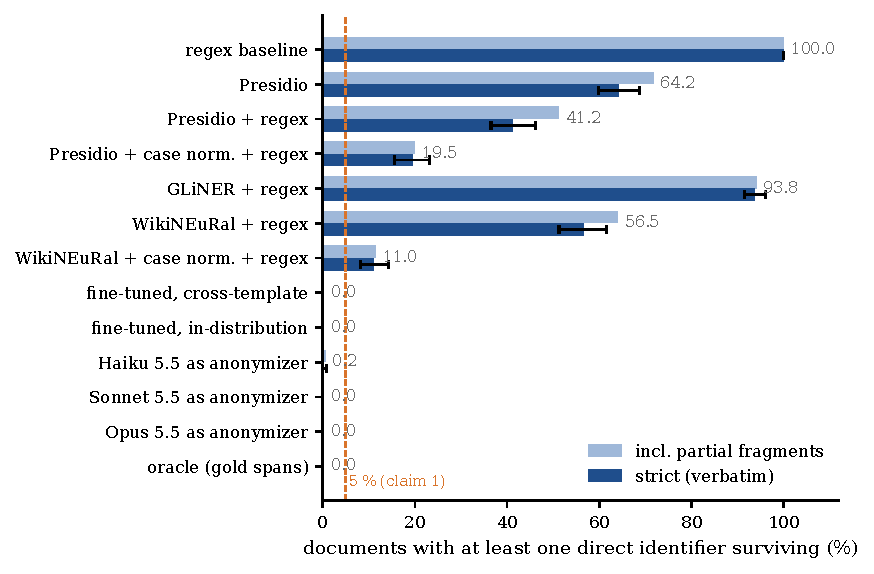
\includegraphics[width=0.92\textwidth]{figures/leak_systems}
\caption{Document leak rate on the test split ($N=400$), typed pseudonyms, policy \textsc{direct+org+loc}: share of documents in which at least one direct identifier survives verbatim (dark) or as a discriminating fragment (light), with 95\,\% cluster-bootstrap CIs. The dashed line is the 5\,\% threshold of the first pre-specified claim.}
\label{fig:leak-systems}
\end{figure}

\paragraph{Headline (Table~\ref{tab:headline}, Figure~\ref{fig:leak-systems}).} With typed pseudonyms and the default policy, Presidio alone leaves at least one direct identifier in 64.2\,\% of test documents (CI 59.8--68.8); adding validated patterns brings this to 41.2\,\% (36.5--46.2), and to 51.2\,\% (46.5--56.2) when discriminating fragments count. The direct-mention leak rate of the hybrid is 7.1\,\% (6.1--8.2), a number that would look acceptable in a recall table and that still means two documents in five reach the provider with a name in them. The regex baseline is at the floor for names (100\,\% of documents) while being perfect on structured identifiers, which is the point: the structured part of Italian PII is solved, the unstructured part is not.

\paragraph{It is the names (Table~\ref{tab:percat}).} For the hybrid, every structured category is at 0\,\% strict leak (rule-of-three bound $\le 3/n$, i.e.\ $<0.7\,\%$ for \pseud{CF}, $<1.2\,\%$ for \pseud{IBAN}). \pseud{PER} leaks at 18.2\,\% of mentions (15.7--20.8), 30.0\,\% (26.9--33.4) including surviving surnames, and 18.9\,\% of person \emph{entities}: one named person in five is still identifiable. Presidio alone additionally leaks addresses (13.1\,\%), dates of birth (14.1\,\%), phones (8.7\,\%), partite IVA (27.0\,\%) and plates (90.0\,\%), all of which the patterns fix. Among quasi-identifiers that the policy does replace, cities (\pseud{LOC}) leak at 25.2\,\% and organisations at 25.0\,\%, including every company name with an \emph{S.r.l.}/\emph{S.p.A.}\ suffix that spaCy did not tag.

\begin{figure}[t]
\centering
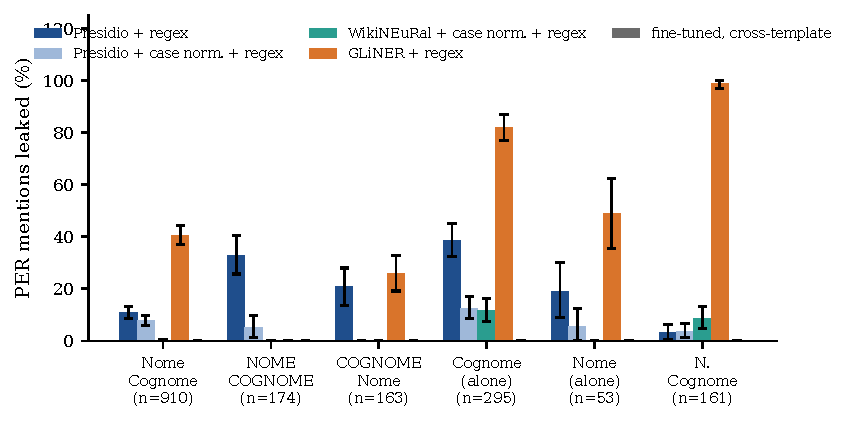
\includegraphics[width=0.92\textwidth]{figures/forms}
\caption{Where the names leak: strict leak rate of \pseud{PER} mentions by surface form for four local detectors (typed, \textsc{direct+org+loc}; $n$ = mentions in the test split). Presidio fails on all-caps and surname-only forms; case normalization removes the all-caps and \emph{COGNOME Nome} failures; GLiNER fails on surnames and initials; the cross-template fine-tuned encoder is the trained reference.}
\label{fig:forms}
\end{figure}

\paragraph{Which names (Table~\ref{tab:forms}, Figure~\ref{fig:forms}).} The leak is orthographic. Canonical \emph{Nome Cognome} mentions leak at 10.9\,\%; surname-only mentions (\emph{la sig.ra Ferraro}, \emph{il ricorrente Massari}) at 38.6\,\%; all-caps names at 32.8\,\%; \emph{COGNOME Nome}, the form of every Italian court file, HR record and hospital header, at 20.9\,\%; first names alone at 18.9\,\%. The spaCy NER was trained on news text where names are mixed-case and in natural order. By domain, clinical (54\,\%) and HR (53\,\%) documents leak twice as often as legal (27\,\%) and financial (31\,\%), because they are the domains that refer to the subject by first name or by title and surname.

\paragraph{Case normalization halves the leak without any training.} Rewriting \emph{COGNOME Nome} as \emph{Nome Cognome} and title-casing all-caps words before the detector sees the text brings the document leak rate of Presidio + regex from 41.2\,\% to 19.5\,\% [15.5, 23.2] and the direct-mention leak rate from 7.1\,\% to 2.8\,\% [2.2, 3.5]. By form, \emph{COGNOME Nome} goes from 20.9\,\% to 0.0\,\%, all-caps from 32.8\,\% to 5.2\,\%, surname-only from 38.6\,\% to 12.5\,\% (a bare surname is found far more often once the full name earlier in the document has been found and the two are linked); by domain, legal and financial documents fall to 4\,\% and 3\,\%, HR to 29\,\% and clinical to 42\,\%, where the surviving mentions are bare surnames in ward prose. The price is 1.4 more spurious replacements per 1\,000 tokens (17.3 against 15.9), from acronyms the title-casing turns into words. The quasi-identifier profile and $\hat k$ do not move, because the policy, not the detector, decides what survives of age and profession. The same preprocessing does more for a supervised multilingual NER model: WikiNEuRal + regex leaks in 56.5\,\% [51.2, 61.5] of documents on the raw text (it finds \emph{Nome Cognome} at 91\,\% but no all-caps name at all) and in 11.0\,\% [8.2, 14.2] after case normalization, with a direct-mention leak rate of 1.2\,\% [0.8, 1.5] and 5.1 spurious replacements per 1\,000 tokens, a third of Presidio's. What remains at 11\,\% is bare surnames (11.9\,\%) and \emph{N.~Cognome} initials (8.7\,\%), concentrated in HR letters and financial reports. The ordering of the local options is therefore preprocessing first, then the choice of NER model, then training: the first two together take the standard stack from two documents in five to one in nine without a single labelled example.

\paragraph{Policy matters more than detector tuning.} Restricting replacement to direct categories raises the document leak rate from 41\,\% to 54\,\% with the same detector, because mis-typed detections (a surname tagged \pseud{LOC}, an all-caps name tagged \pseud{ORG}) stop protecting. Over-redaction moves the other way: 15.9 spurious replacements per 1\,000 tokens under the default policy (\emph{Sede}, \emph{Prot.}, \emph{IBAN} tagged as locations), 3.5 under \textsc{direct\_only}. A deployment that trusts the type of a detection to decide whether to replace it is trading leak for utility in the wrong direction.

\begin{figure}[t]
\centering
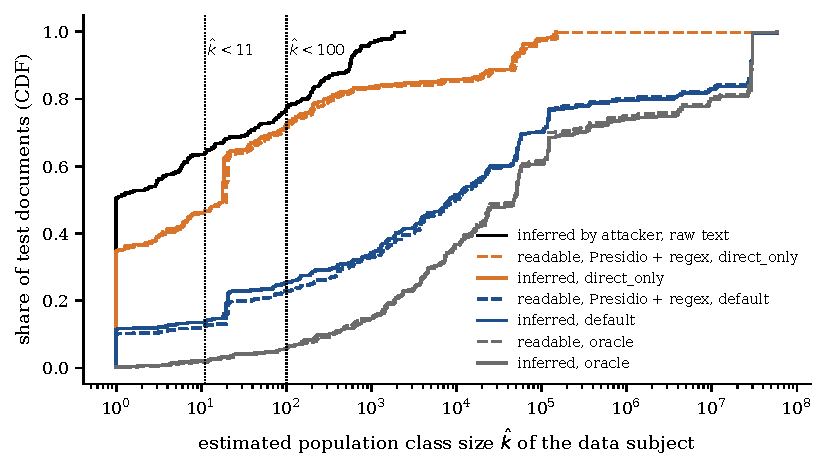
\includegraphics[width=0.92\textwidth]{figures/khat}
\caption{Distribution of the estimated population class size $\hat k$ of the data subject (cumulative share of test documents, log scale). Dashed: computed from the quasi-identifiers still readable in $\dprime$; solid: computed from what the Opus~5.5 attacker infers correctly. The two estimates coincide for every condition; the policy, not the attacker, moves the curve.}
\label{fig:khat}
\end{figure}

\paragraph{Re-identification from what survives (Table~\ref{tab:kanon}, Figure~\ref{fig:khat}).} Under the default policy, age (69\,\%), profession (67\,\%), nationality (26\,\%), marital status (21\,\%) and diagnosis (25\,\%, clinical) survive by design and employer (15\,\%) and city (5\,\%) by failure. The surviving tuple is unique within the 400-document corpus for 79\,\% of subjects. The population estimate $\hat k$ has a median above 10\,000, since most documents expose only coarse attributes, but a long lower tail: the 10th percentile is 1, 12.5\,\% of subjects fall below $\hat k<11$ and 23\,\% below 100. The tail is where employer or city survived together with age and profession. Per domain the median $\hat k$ is about 1\,160 in clinical and 420 in HR documents against $1.2\times10^5$ in legal ones, and in HR 21\,\% of subjects are below 11. Our fourth pre-specified claim (median $\hat k<100$ for HR and clinical) is therefore \emph{not} supported; the risk is in the tail, not the median, which is the argument for reporting the distribution. The oracle shows the floor of the metric at this policy: even with perfect direct-identifier removal, 1.8\,\% of subjects are below 11 from age, profession and diagnosis alone, and 83\,\% of clinical equivalence classes contain a single diagnosis ($l=1$).

\paragraph{Zero-shot NER is worse; a trained encoder leaks nothing on this benchmark, and that is partly the benchmark (Table~\ref{tab:llmself}).} GLiNER with Italian labels and regex leaves a direct identifier in 93.8\,\% [91.5, 96.0] of documents: it finds 100\,\% of ALL-CAPS names and 60\,\% of \emph{Nome Cognome} mentions but only 18\,\% of bare surnames and 1\,\% of \emph{N.~Cognome} forms, so almost every document keeps at least one. English labels do not help (99\,\% on a 100-document subsample); lowering the threshold to 0.25 brings the document rate to 85\,\% [78, 91] at the cost of more over-redaction. The supervised WikiNEuRal model sits in between on raw text (56.5\,\%) and, as shown above, becomes the best off-the-shelf option once the input is case-normalized. At the other end, a BERT encoder fine-tuned on the 1\,400 train documents leaks 0.0\,\% (rule of three: $<0.75$\,\%) with 1.4 spurious replacements per 1\,000 tokens. We do not read this as a result: train and test share template families and a closed vocabulary, so the tagger can learn positions rather than names. The cross-template check (train on two domains, evaluate on the other two, both folds) still leaks 0.0\,\% of documents, which says that the surface forms of Italian names transfer across document types, but its over-redaction rises from 1.4 to 31.0 spurious replacements per 1\,000 tokens: a model that has never seen a clinical letter still finds every name in it and also replaces a great deal that is not one. The honest summary is that training closes the leak and opens an over-redaction cost that the in-distribution number hides; how much of either survives real orthography is a question only real documents can answer (\S\ref{sec:limits}).

% auto-generated by scripts/make_frontier_tables.py — do not edit by hand
\begin{table*}[t]\centering\small
\caption{Downstream quality on the test split. Raw rows give absolute accuracy (\%); pseudonymized rows give $\Delta$ = quality(condition) $-$ quality(raw) in points with 95\,\% paired-bootstrap CIs over documents (pre-registered non-inferiority margin: 2 points). The pairwise summary judge is reported in the text only (\S\ref{sec:results}), since its preference is an artifact of identifier completeness. Agr.\ = heuristic agreement-error rate on the pseudonymized summaries (\S\ref{sec:downstream}). Pseudonymizer: Presidio + regex unless \textsc{oracle}.}
\label{tab:downstream}
\begin{adjustbox}{max width=\textwidth}
\begin{tabular}{llrrrrr}\toprule
Consumer & condition & $N$ & QA & classify & extract & agr.\ err.\ \% \\ \midrule
Opus 5.5, medium & raw & 400 & 100.0 & 94.5 & 98.8 & -- \\
 & typed (\textsc{d+o+l}) & 400 & -0.4 [-1.0, +0.0] & -3.8 [-6.2, -1.2] & -2.5 [-4.0, -1.0] & 2.6 [1.0, 4.3] \\
 & opaque (\textsc{d+o+l}) & 400 & +0.0 [+0.0, +0.0] & -3.0 [-5.5, -0.2] & -3.5 [-5.4, -1.7] & 4.9 [2.7, 7.1] \\
 & typed (\textsc{direct\_only}) & 400 & +0.0 [+0.0, +0.0] & -1.8 [-4.0, +0.5] & -1.7 [-3.1, -0.5] & 3.9 [2.1, 5.9] \\
 & typed (\textsc{all}) & 400 & -0.1 [-0.4, +0.0] & -3.0 [-5.5, -0.5] & -2.6 [-4.1, -1.0] & 5.4 [3.2, 7.7] \\
 & oracle typed (\textsc{d+o+l}) & 400 & +0.0 [+0.0, +0.0] & +1.8 [+0.0, +3.8] & +0.0 [-0.4, +0.4] & 4.8 [2.9, 6.9] \\
\midrule
Opus 5.5, low & raw & 400 & 100.0 & 92.8 & 98.7 & -- \\
 & typed (\textsc{d+o+l}) & 400 & +0.0 [+0.0, +0.0] & -3.8 [-6.5, -1.0] & -2.5 [-4.1, -1.0] & 4.0 [2.1, 6.1] \\
 & opaque (\textsc{d+o+l}) & 400 & -0.1 [-0.4, +0.0] & -4.0 [-7.0, -1.0] & -3.7 [-5.6, -1.8] & 4.9 [2.8, 7.0] \\
\midrule
Opus 5.5, high & raw & 100 & 100.0 & 96.0 & 99.1 & -- \\
 & typed (\textsc{d+o+l}) & 100 & +0.0 [+0.0, +0.0] & -4.0 [-9.0, +1.0] & -2.0 [-5.1, +0.0] & 3.3 [0.0, 7.1] \\
\midrule
Sonnet 5.5, medium & raw & 400 & 100.0 & 87.0 & 98.7 & -- \\
 & typed (\textsc{d+o+l}) & 400 & -0.1 [-0.4, +0.0] & -2.8 [-5.8, +0.2] & -5.6 [-7.7, -3.5] & 3.4 [1.4, 5.7] \\
 & opaque (\textsc{d+o+l}) & 400 & -0.5 [-1.3, +0.0] & -3.8 [-7.0, -0.5] & -5.1 [-7.1, -3.1] & 4.4 [2.2, 6.8] \\
\midrule
Haiku 5.5, medium & raw & 400 & 100.0 & 82.2 & 98.4 & -- \\
 & typed (\textsc{d+o+l}) & 400 & -0.8 [-1.7, -0.1] & -2.0 [-5.0, +0.8] & -4.4 [-6.3, -2.4] & 5.6 [3.2, 8.5] \\
 & opaque (\textsc{d+o+l}) & 400 & -1.3 [-2.4, -0.4] & -1.2 [-3.8, +1.2] & -5.4 [-7.6, -3.4] & 4.3 [2.2, 6.5] \\
\bottomrule\end{tabular}\end{adjustbox}\end{table*}

\begin{table}[t]\centering\small
\caption{Run-to-run variance of $\Delta$(typed) for the Opus 5.5 consumer: the primary run and repeat runs with a fresh cache salt (points, 95\,\% CI). The spread across runs is the sampling noise of the model itself and should be read next to the bootstrap CI, which only captures document sampling.}
\label{tab:variance}
\begin{adjustbox}{max width=\textwidth}
\begin{tabular}{lrrrr}\toprule Run & $N$ & QA & classify & extract \\ \midrule
primary, 400 & 400 & -0.4 [-1.0, +0.0] & -3.8 [-6.2, -1.2] & -2.5 [-4.0, -1.0] \\
rep3, 400 & 400 & -0.4 [-1.0, +0.0] & -3.0 [-5.8, -0.2] & -2.4 [-4.0, -1.0] \\
rep1, 100 & 100 & +0.0 [+0.0, +0.0] & -6.0 [-12.0, -1.0] & -2.0 [-5.1, +0.0] \\
rep2, 100 & 100 & +0.0 [+0.0, +0.0] & -5.0 [-10.0, +0.0] & -2.0 [-5.1, +0.0] \\
\bottomrule\end{tabular}\end{adjustbox}\end{table}

\begin{table}[t]\centering\small
\caption{Pairwise summary judge on the Opus~5.5 consumer run: share of documents in which the judge prefers the reverse-mapped pseudonymized summary over the raw-input summary (ties count one half, both presentation orders, 95\,\% bootstrap CI over documents; 0.5 = parity). The default prompt rewards identifier completeness (\S\ref{sec:results}); the completeness-blind prompt tells the judge to ignore how many names, codes and addresses a summary carries.}
\label{tab:judge}
\begin{adjustbox}{max width=\textwidth}
\begin{tabular}{llrrr}\toprule Judge & Prompt & typed & opaque & \textsc{oracle} \\ \midrule
Sonnet 5.5 & default & 0.68 [0.64, 0.72] & 0.73 [0.69, 0.76] & 0.75 [0.72, 0.79] \\
Opus 5.5 & default & 0.67 [0.63, 0.71] & 0.72 [0.68, 0.76] & -- \\
Qwen2.5-72B & default & 0.66 [0.63, 0.69] & 0.66 [0.64, 0.69] & -- \\
Qwen2.5-72B & completeness-blind & 0.39 [0.37, 0.41] & 0.40 [0.38, 0.43] & 0.48 [0.46, 0.51] \\
\bottomrule\end{tabular}\end{adjustbox}\end{table}

\begin{table}[t]\centering\small
\caption{LLM-judged agreement (Sonnet 5.5 judge, \S\ref{sec:downstream}). ``Gendered'' = share of person pseudonyms in the summary for which the model produced any gender-marked agreement; error = share of those whose agreement contradicts the gold gender. Cluster-bootstrap CIs over documents.}
\label{tab:agreement-judge}
\begin{adjustbox}{max width=\textwidth}
\begin{tabular}{llrrrr}\toprule Consumer run & condition & pseudonyms & gendered \% & inconsistent & error \% [CI] \\ \midrule
haiku-5-5, medium & typed & 789 & 41 & 2 & 0.6 [0.0, 1.5] \\
haiku-5-5, medium & opaque & 747 & 22 & 3 & 1.9 [0.0, 4.4] \\
sonnet-5-5, medium & typed & 819 & 43 & 2 & 0.6 [0.0, 1.5] \\
sonnet-5-5, medium & opaque & 801 & 24 & 2 & 1.0 [0.0, 2.7] \\
\bottomrule\end{tabular}\end{adjustbox}\end{table}

\begin{table*}[t]\centering\small
\caption{The frontier model as its own anonymizer (\texttt{llm\_self}, one call per document asking for all identifier mentions) against the local systems, same policy and metrics as Table~\ref{tab:headline}. Not a deployable option (the provider sees the raw text): it bounds what a local detector forgoes.}
\label{tab:llmself}
\begin{adjustbox}{max width=\textwidth}
\begin{tabular}{lrrrrrr}\toprule System & $N$ & doc.\ leak \% & incl.\ partial & \texttt{PER} leak & over-red.\ & $\hat k<11$ \\ \midrule
\texttt{presidio} & 400 & 64.2 [59.8, 68.8] & 71.8 [67.2, 76.0] & 17.5 [15.1, 20.1] & 15.9 & 13\,\% \\
\texttt{presidio+regex} & 400 & 41.2 [36.5, 46.2] & 51.2 [46.5, 56.2] & 18.2 [15.7, 20.8] & 15.9 & 12\,\% \\
\texttt{presidio+casenorm+regex} & 400 & 19.5 [15.5, 23.2] & 20.0 [16.0, 23.8] & 7.2 [5.5, 8.9] & 17.3 & 12\,\% \\
\texttt{wikineural+regex} & 400 & 56.5 [51.2, 61.5] & 64.0 [59.0, 68.8] & 29.6 [26.5, 32.5] & 4.5 & 9\,\% \\
\texttt{wikineural+casenorm+regex} & 400 & 11.0 [8.2, 14.2] & 11.5 [8.5, 14.8] & 2.8 [2.0, 3.7] & 5.1 & 8\,\% \\
\texttt{gliner+regex} & 400 & 93.8 [91.5, 96.0] & 94.0 [91.8, 96.2] & 47.7 [45.6, 49.9] & 3.9 & 13\,\% \\
\texttt{finetuned+regex} & 400 & 0.0 [0.0, 0.0] & 0.2 [0.0, 0.8] & 0.0 [0.0, 0.0] & 1.4 & 2\,\% \\
\texttt{finetuned-xt+regex} & 400 & 0.0 [0.0, 0.0] & 0.2 [0.0, 0.8] & 0.0 [0.0, 0.0] & 31.0 & 2\,\% \\
\texttt{llm\_self-haiku-5-5-low} & 400 & 0.2 [0.0, 0.8] & 0.5 [0.0, 1.2] & 0.0 [0.0, 0.0] & 4.7 & 2\,\% \\
\texttt{llm\_self-opus-5-5-low} & 400 & 0.0 [0.0, 0.0] & 0.2 [0.0, 0.8] & 0.0 [0.0, 0.0] & 0.3 & 2\,\% \\
\texttt{llm\_self-opus-5-5-medium} & 400 & 0.0 [0.0, 0.0] & 0.2 [0.0, 0.8] & 0.0 [0.0, 0.0] & 1.6 & 2\,\% \\
\texttt{llm\_self-sonnet-5-5-low} & 400 & 0.0 [0.0, 0.0] & 0.2 [0.0, 0.8] & 0.0 [0.0, 0.0] & 4.2 & 2\,\% \\
\texttt{oracle} & 400 & 0.0 [0.0, 0.0] & 0.2 [0.0, 0.8] & 0.0 [0.0, 0.0] & 0.0 & 2\,\% \\
\bottomrule\end{tabular}\end{adjustbox}\end{table*}

\begin{table*}[t]\centering\small
\caption{LLM attacker (Opus~5.5 unless stated, \S\ref{sec:attacker}): recall (\%) of the data subject's attributes inferred from the text the consumer model receives, surname recovery, and the population $\hat k$ recomputed on the correctly inferred attributes (same marginals as Table~\ref{tab:kanon}). Raw text is the ceiling; \textsc{oracle} isolates what the text reveals once every gold span is replaced.}
\label{tab:attacker}
\begin{adjustbox}{max width=\textwidth}
\begin{tabular}{lrrrrrrrrrrrr}\toprule
Condition & gender & age & city & profession & employer & nationality & marital status & diagnosis & surname & med.\ $\hat k$ & $\hat k<11$ & $\hat k<100$ \\ \midrule
raw text (ceiling) & 100 & 100 & 88 & 66 & 90 & 90 & 26 & 100 & 100.0 & 1 & 64\,\% & 77\,\% \\
typed d+o+l & 100 & 69 & 2 & 66 & 36 & 35 & 25 & 100 & 35.0 & 8,295 & 14\,\% & 26\,\% \\
opaque d+o+l & 100 & 69 & 3 & 66 & 36 & 32 & 25 & 100 & 36.0 & 7,937 & 14\,\% & 26\,\% \\
typed direct\_only & 100 & 69 & 88 & 66 & 86 & 74 & 25 & 100 & 47.2 & 18 & 46\,\% & 72\,\% \\
typed all & 100 & 68 & 3 & 66 & 36 & 34 & 25 & 100 & 35.0 & 8,769 & 14\,\% & 25\,\% \\
oracle typed d+o+l & 100 & 68 & 0 & 66 & 0 & 10 & 26 & 100 & 0.0 & 47,287 & 2\,\% & 6\,\% \\
typed d+o+l, Sonnet attacker & 100 & 69 & 2 & 66 & 36 & 26 & 26 & 100 & 34.8 & 8,399 & 14\,\% & 26\,\% \\
typed d+o+l, Qwen2.5-14B attacker (local) & 98 & 64 & 2 & 64 & 24 & 26 & 26 & 99 & 31.5 & 19,429 & 11\,\% & 19\,\% \\
raw text, Qwen2.5-14B attacker (100 docs) & 100 & 98 & 79 & 67 & 92 & 47 & 31 & 100 & 100.0 & 1 & 65\,\% & 82\,\% \\
oracle, Qwen2.5-14B attacker (100 docs) & 97 & 68 & 0 & 67 & 0 & 0 & 30 & 96 & 0.0 & 33,380 & 1\,\% & 8\,\% \\
typed d+o+l, Qwen2.5-72B attacker (RunPod) & 98 & 68 & 2 & 66 & 26 & 26 & 26 & 99 & 33.8 & 15,342 & 12\,\% & 20\,\% \\
opaque d+o+l, Qwen2.5-72B attacker & 93 & 68 & 3 & 67 & 35 & 26 & 26 & 100 & 34.8 & 9,531 & 14\,\% & 25\,\% \\
typed direct\_only, Qwen2.5-72B attacker & 100 & 67 & 83 & 65 & 84 & 26 & 26 & 100 & 45.0 & 20 & 44\,\% & 71\,\% \\
raw text, Qwen2.5-72B attacker & 100 & 100 & 84 & 67 & 90 & 26 & 28 & 100 & 100.0 & 1 & 64\,\% & 77\,\% \\
oracle, Qwen2.5-72B attacker & 100 & 69 & 0 & 66 & 0 & 0 & 28 & 100 & 0.0 & 45,929 & 2\,\% & 6\,\% \\
\bottomrule\end{tabular}\end{adjustbox}\end{table*}

\begin{table}[t]\centering\small
\caption{Readable versus inferable (typed, \textsc{direct+org+loc}, Presidio + regex): share of data subjects whose attribute is still readable verbatim in $d'$ against the share the Opus~5.5 attacker infers correctly, both among documents where the attribute applies.}
\label{tab:readable-inferable}
\begin{adjustbox}{max width=\textwidth}
\begin{tabular}{lrrr}\toprule Attribute & readable \% & inferred \% & precision \% \\ \midrule
gender & 100 & 100 & 100 \\
age & 69 & 69 & 100 \\
city & 5 & 2 & 8 \\
profession & 67 & 66 & 98 \\
employer & 30 & 36 & 100 \\
nationality & 26 & 35 & 99 \\
marital status & 21 & 25 & 93 \\
diagnosis & 100 & 100 & 100 \\
\bottomrule\end{tabular}\end{adjustbox}\end{table}



\paragraph{The frontier model as its own anonymizer (Table~\ref{tab:llmself}).} Asked for every identifier mention in one call, Opus~5.5 (effort low or medium) and Sonnet~5.5 leak 0.0\,\% of documents and Haiku~5.5 0.2\,\% [0.0, 0.8], with 0.3--4.7 spurious replacements per 1\,000 tokens; the surviving quasi-identifier profile is the oracle's (1.8\,\% of subjects with $\hat k<11$). The comparison that the deployment question turns on is therefore stark: the local off-the-shelf stack leaves a name in two documents out of five, the provider's own model in none; but the provider's model has, by construction, already seen the name. This does not make the option unusable. Under a processor contract with zero data retention the raw text is processed, not retained, and the result above says the processor's own anonymization is the most accurate one available. What the result changes is the nature of the question: whether to trust the provider with the raw text is then a contractual and supervisory decision (Art.~28, the DPA, the audit rights), not a measurement, and the local pseudonymizer is the option for organisations that cannot or will not take it. For those, on this benchmark, the privacy argument rests on a trained detector, with the caveats of \S\ref{sec:limits} about what the synthetic benchmark can show.

\paragraph{What the recipient can infer (Table~\ref{tab:attacker}).} The Opus~5.5 attacker recovers the subject's surname from 100\,\% of raw documents, from 35.0\,\% of typed documents under the default policy (the names Presidio missed: the figure tracks the 41\,\% document leak rate, less the cases where the surviving mention is an initial or a fragment the attacker does not commit to), from 47.2\,\% under \textsc{direct\_only}, and from 0.0\,\% after the oracle. On the attributes, the attacker reads what is readable and little more (Table~\ref{tab:readable-inferable}): recall equals surface survival for gender, age and profession, and exceeds it by 6--9 points for employer and nationality, which it infers from context rather than reads; precision is above 93\,\% for every attribute except city, which the policy removes. The inference-based $\hat k$ moves accordingly: 64\,\% of subjects are in a class of fewer than 11 on raw text, 47\,\% under \textsc{direct\_only}, 14\,\% under the default policy (the surface estimate gives 12.5\,\%), 2\,\% after the oracle; with WikiNEuRal and case normalization the surface estimate is 8.2\,\%. Removing quasi-identifiers beyond the default (\textsc{all}) changes nothing, because the attributes that survive, age and profession, are stated in the running text in forms the detector does not tag. A weaker attacker from the same provider (Sonnet~5.5) recovers the same surnames (34.8\,\%) and the same $\hat k$ distribution, and so do two open-weight models from another house. Qwen2.5-14B-Instruct, run locally, recovers 31.5\,\% of surnames on the typed condition, 100\,\% on raw text and 0\,\% after the oracle, with 10.8\,\% of subjects below $\hat k<11$ (Opus: 14\,\%). Qwen2.5-72B-Instruct, run on every condition, lands within two points of Opus everywhere: 33.8\,\% of surnames typed, 34.8\,\% opaque, 45.0\,\% under \textsc{direct\_only}, 33.5\,\% under \textsc{all}, 100\,\% raw and 0\,\% oracle, with 12\,\%, 14\,\%, 45\,\%, 12\,\%, 64\,\% and 1.8\,\% of subjects below $\hat k<11$ respectively. The result is a property of the text, not of the attacker's strength or provenance.

\begin{figure}[t]
\centering
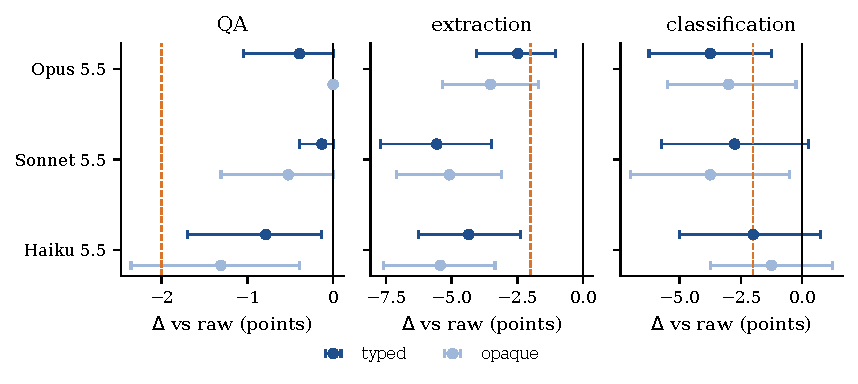
\includegraphics[width=0.95\textwidth]{figures/downstream}
\caption{Downstream quality: $\Delta$ = quality(pseudonymized) $-$ quality(raw) in points, typed and opaque pseudonyms, three consumer models, 95\,\% paired-bootstrap CIs over documents. Dashed: the pre-specified two-point non-inferiority margin.}
\label{fig:downstream}
\end{figure}
\begin{figure}[t]
\centering
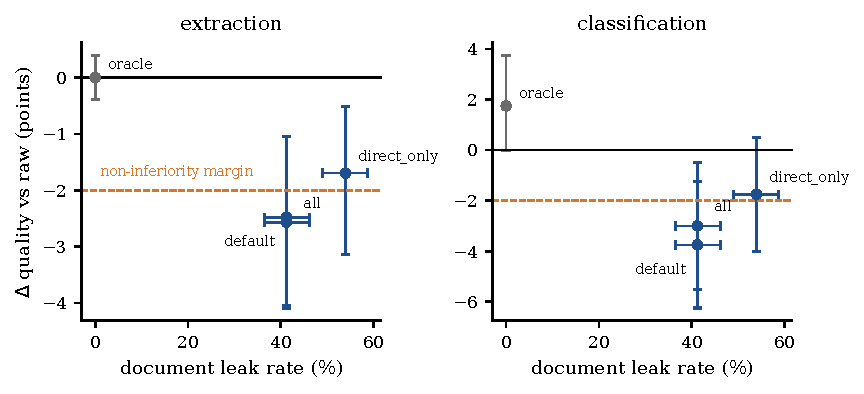
\includegraphics[width=0.95\textwidth]{figures/privacy_utility}
\caption{The privacy--utility plane for the Opus~5.5 consumer: document leak rate of each replacement policy (Presidio + regex, typed) against its $\Delta$ on extraction and classification. The \pseud{oracle} point (gold spans replaced) sits at zero leak and zero loss: the loss of the other points is the detector's.}
\label{fig:privacy-utility}
\end{figure}

\paragraph{Downstream quality: the loss is the detector's, not the pseudonym's (Table~\ref{tab:downstream}, Figures~\ref{fig:downstream} and \ref{fig:privacy-utility}).} With Opus~5.5 as the consumer, typed pseudonyms under the default policy cost $-0.4$ points [$-1.0$, $0.0$] on QA, $-2.5$ [$-4.0$, $-1.0$] on extraction and $-3.8$ [$-6.2$, $-1.2$] on classification; the pre-specified two-point non-inferiority margin holds for QA only. The \pseud{oracle} condition (gold spans replaced, nothing else changed) gives $0.0$ [$-0.4$, $+0.4$] on extraction and $+1.8$ [$0.0$, $+3.8$] on classification. The entire loss is therefore attributable to detection errors: Presidio replaces a CCNL name or a diagnosis it has taken for an organisation, and the model, told to copy placeholders verbatim, returns \emph{null} for a field it can no longer read. Reverse mapping itself fails on 0.0--0.2\,\% of pseudonym tokens. Across policies the ordering is as expected (\textsc{direct\_only} $-1.7$, default $-2.5$, \textsc{all} $-2.6$ on extraction), with no measurable difference between typed and opaque pseudonyms on any task. Smaller consumers lose more on extraction (Sonnet~5.5 $-5.6$ [$-7.7$, $-3.5$], Haiku~5.5 $-4.4$ [$-6.3$, $-2.4$]) and Haiku is the only model whose QA drops measurably ($-0.8$ [$-1.7$, $-0.1$]); effort level does not matter (Opus low: $-2.5$ on extraction; high, 100 documents: $-2.0$ [$-5.1$, $0.0$]). No request was refused and no output hit the token limit.

\paragraph{The summary judge is an artifact of its prompt (Table~\ref{tab:judge}).} The pairwise judge, shown the raw document and both summaries, prefers the reverse-mapped pseudonymized summary in 65--75\,\% of documents (Opus as a second judge agrees: 0.67 typed, 0.72 opaque; Qwen2.5-72B with the same prompt: 0.66 and 0.66), and prefers the \pseud{oracle} summary most of all (0.75). We keep this number out of Table~\ref{tab:downstream} because it is not a quality measurement. The instruction to copy placeholders verbatim makes the model carry identifiers into the summary that it would otherwise paraphrase or drop: after reverse mapping, pseudonymized summaries contain 48\,\% of the document's gold direct identifiers against 31\,\% for raw summaries, and are 5\,\% longer; the judge rewards the completeness. Telling the judge to ignore how many names, codes and addresses a summary carries reverses the verdict: the same Qwen2.5-72B judge then prefers the pseudonymized summary in 39\,\% of documents (typed) and 40\,\% (opaque), and the \pseud{oracle} summary in 48.5\,\%, that is, at parity. Three readings follow. The 0.66--0.75 preference is a property of the prompt, not of the judge model, since three judges from two houses reproduce it. Once completeness is discounted, summaries written from Presidio-pseudonymized text sit about ten points of pairwise preference below raw, in line with the two-to-four-point losses on the other tasks. And the oracle at parity places that loss where the extraction and classification losses already were: in the detector's mistakes, not in the pseudonyms.

\paragraph{Variance across runs (Table~\ref{tab:variance}).} Repeating the typed condition on the full split with a fresh cache salt reproduces every $\Delta$ within 0.8 points ($-3.0$ against $-3.8$ on classification, $-2.4$ against $-2.5$ on extraction); the two 100-document repeats sit inside the full-split CIs. The bootstrap CI over documents is therefore not understating the uncertainty by much on this corpus; model sampling noise is second-order.

\begin{figure}[t]
\centering
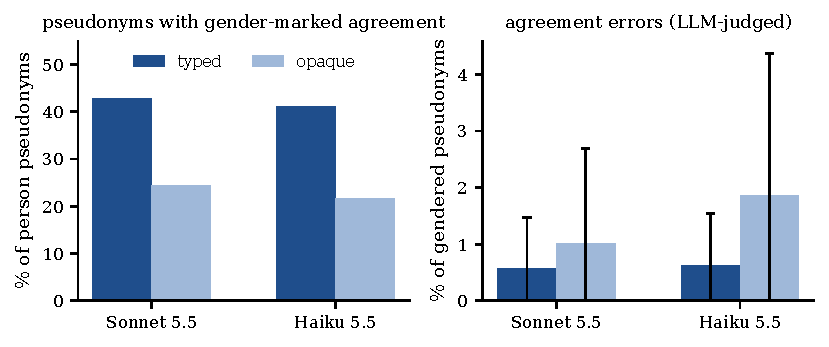
\includegraphics[width=0.9\textwidth]{figures/agreement}
\caption{LLM-judged grammatical agreement on the summaries. Left: share of person pseudonyms for which the model produced any gender-marked agreement. Right: share of those whose agreement contradicts the gold gender, with 95\,\% CIs. Typed pseudonyms change the left panel, not the right one.}
\label{fig:agreement}
\end{figure}

\paragraph{Typed pseudonyms make the model commit to a gender; they do not make it wrong (Table~\ref{tab:agreement-judge}, Figure~\ref{fig:agreement}).} The judged agreement-error rate is 0.6\,\% for typed and 1.0\,\% (Sonnet) or 1.9\,\% (Haiku) for opaque pseudonyms, with two to three inconsistent pseudonyms out of about 800 in each run; the heuristic checker, which also sees the Opus runs, gives 2.6\,\% [1.0, 4.3] typed against 4.9\,\% [2.7, 7.1] opaque. The pre-specified claim, a halving of errors, cannot be established at these rates and we do not claim it. What the data show instead is that with opaque pseudonyms the model avoids gender altogether: 41--43\,\% of person pseudonyms receive gender-marked agreement (\emph{la sig.ra [[x]], convocata}) when the pseudonym carries the gender, 22--24\,\% when it does not. Typed pseudonyms buy natural Italian, not fewer errors. A separate source of error sits upstream: 3.8\,\% of typed person pseudonyms carry the wrong gender, because the pseudonymizer had to infer it from a surname-only mention; a consumer that follows the tag faithfully then produces agreement that is consistent with the pseudonym and wrong about the person.

\clearpage
\section{GDPR status of the pipeline and what a DPIA must document}
\label{sec:gdpr}

\paragraph{Pseudonymization, not anonymization.} Replacing identifiers with tokens while keeping a mapping is pseudonymization in the sense of Art.~4(5) GDPR \citep{gdpr2016}: the data ``can no longer be attributed to a specific data subject without the use of additional information'' which is ``kept separately and \ldots subject to technical and organisational measures''. Pseudonymized data remain personal data for the controller (Recital~26). The Article~29 Working Party's position \citep{wp29anon2014} was that they remain personal data for everyone. The EDPB's draft Guidelines 01/2025 \citep{edpb2025pseudonymisation} treat pseudonymization as a risk-reduction measure under Arts.~25 and 32 and spell out what the ``additional information'' must look like: the mapping (or key) separated from the data, access-controlled, with the pseudonymization domain defined so that the recipient cannot attribute the data. The pipeline studied here is exactly this architecture, with $M$ on premise, \emph{provided the pseudonymization actually worked}. A $\dprime$ that still contains the subject's name is not pseudonymized data; it is personal data transmitted to a processor, with every consequence of Arts.~28 and 44 ff.\ that the deployment was meant to avoid. The leak rate is therefore not a quality metric; it is the share of transmissions for which the legal characterisation the DPIA relies on is false.

\paragraph{The relative reading after \emph{EDPS v SRB}.} On 4 September 2025 the Court of Justice set aside the General Court's judgment in \emph{SRB v EDPS} (T-557/20) and held, in C-413/23~P \citep{cjeu2025srb}, that pseudonymized data need not be regarded as personal data for every person in every case: whether they are personal data for a given recipient depends on whether that recipient has reasonably likely means of re-identification, in the \emph{Breyer} sense \citep{cjeu2016breyer}, while they remain personal data for the controller who holds the key, and while the controller's transparency duties towards data subjects are assessed from the controller's perspective and are unaffected. Read for our pipeline: the frontier provider that receives a \emph{correctly} pseudonymized $\dprime$ may not be processing personal data at all, which is the strongest possible position for the deploying organisation. The judgment makes the measurement in this paper more important, not less: the relative reading is available only for data in which the recipient has no reasonably likely means of attribution, and a document in which the name survives, or in which the surviving quasi-identifier tuple has $\hat k$ of a few units, hands the recipient exactly such means. Two cautions follow from the judgment's own limits: the characterisation is per recipient, so it must be re-done if the provider passes data on or combines it with other sources; and nothing in it relaxes the controller's obligations, so the DPIA, the processor contract and the information to data subjects remain due.

\paragraph{What the DPIA (Art.~35) must contain.} The measurement framework maps onto the DPIA's required content. \emph{Systematic description of the processing}: the pipeline diagram of \S\ref{sec:defs}, the categories replaced (the replacement policy), the mapping schema and where $M$ is stored. \emph{Necessity and proportionality}: the over-redaction rate and the downstream $\Delta$ answer why the chosen policy does not remove more. \emph{Assessment of the risks}: the document leak rate with its CI, per category and per domain, is the probability that a transmission contains direct identifiers; the $\hat k$ distribution is the residual singling-out risk from what the policy deliberately keeps; both must be measured on the organisation's own document types, not on a benchmark. \emph{Measures envisaged}: the detector configuration and its validation report, the handling of refusals and reverse-mapping failures, re-measurement on model or policy change, and, because the leak concentrates in predictable forms, pre-processing rules for all-caps and \emph{COGNOME Nome} headers. A DPIA that reports NER F1 instead of these quantities has not assessed the risk it describes.

\section{Limitations}
\label{sec:limits}
The benchmark is synthetic (\S\ref{sec:data}): absolute rates are lower bounds for real documents, and the vocabulary is closed. The population marginals behind $\hat k$ are ISTAT tables where ISTAT publishes them (population, sex, age bands, civil status, citizenship, municipalities) and ISTAT-derived approximations for the fine occupation and diagnosis shares, rounded and listed with their sources in the released reference table; the estimator assumes independence between attributes, which it does not hold, so the distribution shape, not the point values, is the finding. Gender is treated as always surviving, which is conservative for opaque pseudonyms in texts without agreement cues. The heuristic agreement checker is lexicon-based and conservative; the judged rate depends on a prompt that was revised twice against inspected verdicts (\S\ref{sec:downstream}), and both versions are reported in the released results. The fine-tuned encoder's 0\,\% is a property of the synthetic data: train and test share template families and a closed vocabulary, so a tagger can learn positions rather than names; the cross-template check (zero leak again, but twenty times the over-redaction) shows that the forms transfer and the precision does not, and neither number says what a model trained on one institution's documents does on another's. The extraction and QA gold was filtered to facts stated in the text after the generator was found to record unrendered fields; the filter is identical across conditions and the full unfiltered scores are in the released results. The judge prefers pseudonymized summaries for a reason we can name (they carry more identifiers back after reverse mapping), and a judge instructed to ignore identifier completeness reverses the preference; that second prompt was written after the bias was diagnosed and run once, so it is a check, not a pre-specified instrument. The three consumer models are from one provider; the attacker and the judge were repeated with open-weight models from another house with the same conclusions, and the harness takes any Messages-API or OpenAI-compatible endpoint, so the consumer side can be repeated elsewhere.

\section{Conclusion}
A local pseudonymizer in front of a frontier API is sold on a sentence, ``no personal data leaves the building'', whose truth value is a measurable rate. We defined that rate, built an Italian benchmark that can measure it, and found that the standard open-source stack leaves a name in two documents out of five while being perfect on every structured identifier; that an attacker reading the pseudonymized text, from either of two model houses, recovers that name just as often and still singles out one subject in eight; that a free preprocessing step, case normalization, halves the leak and takes a supervised multilingual NER model to one document in nine, while zero-shot NER is worse than Presidio and a fine-tuned encoder reaches zero only on a benchmark whose vocabulary it has seen; and that the two-to-four-point downstream loss the pipeline does incur is caused by the detector's mistakes, not by the pseudonyms. Downstream quality, the metric prior work optimised, cannot see any of this. The code and benchmark are released so that the measurement can be repeated where it matters: on the organisation's own documents, before the DPIA is signed.

\section*{Ethics and data statement}
No real personal data were used. All identifiers in the benchmark are synthetic; codici fiscali, IBANs and partite IVA are checksum-valid strings generated from fictitious attributes and do not correspond to real persons or accounts. Names and cities are drawn from public frequency lists.

\bibliographystyle{plainnat}
\bibliography{references}

\appendix
\section{Wilson vs.\ cluster-bootstrap intervals}
For every rate in Table~\ref{tab:percat} the released evaluation files report the mention-level Wilson interval alongside the cluster bootstrap. For Presidio + regex, \pseud{PER}: Wilson 16.4--20.0\,\%, bootstrap 15.7--20.8\,\%; document leak rate (one observation per document, so the two coincide up to sampling): 36.5--46.2\,\%. The understatement grows with the number of mentions per entity.

\section{Mapping schema}
\begin{verbatim}
{"doc_id": "hr_test_00012", "mode": "typed",
 "entries": [
  {"pseudonym": "PER_f_0001", "category": "PER", "canonical": "Giulia Ferraro",
   "surfaces": ["Giulia Ferraro", "FERRARO Giulia", "Ferraro"],
   "attrs": {"gender": "f"}},
  {"pseudonym": "CF_0001", "category": "CF", "canonical": "FRRGLI87S45F205E",
   "surfaces": ["FRRGLI87S45F205E"], "attrs": {}}]}
\end{verbatim}
Reverse mapping is longest-match over pseudonym tokens, tolerant to lower-casing, lost underscores, trailing punctuation and possessives; unresolvable tokens are counted as reverse-mapping failures.

\section{Reproducibility}
{\small
\begin{verbatim}
python -m leakrate generate --n 500
python -m leakrate pseudonymize --system presidio+regex
python -m leakrate evaluate \
    --pseudo results/pseudo/presidio-regex__typed__direct-org-loc__test.jsonl
python -m leakrate report && python scripts/make_tables.py
LANE=opus bash scripts/run_frontier_full.sh    # frontier protocol (needs API key)
LANE=small bash scripts/run_frontier_full.sh
bash scripts/run_frontier_extra.sh              # re-score, agreement judge, tables
\end{verbatim}}

\end{document}
